\section{Ejercicio 4}

\subsection{Introducción}

Para este ejercicio se pedía dado un arreglo de $N$ matrices en
$\mathbb{Z}_{10007}^{3 \times 3}$ decidir si existía un subarreglo de longitud
$L$ tal que su producto fuera igual a $M \in \mathbb{Z}_{10007}^{3 \times 3}$.
Además, el algoritmo desarrollado debía tener una complejidad temporal $\ord(N
\times \log N)$.

\subsection{Solución propuesta}\label{ej4:sol}

La solución desarrollada hace uso de la técnica de \emph{Divide \& Conquer}.
Esto se debe a que el problema tiene la característica de poder ser dividido en
subproblemas más pequeños que unidos resuelven lo pedido.

Si existe el subarreglo cuyo producto corresponde a $M$ es bajo alguna de
las siguientes posibilidades:

\begin{itemize}
	\item El subarreglo existe en $\left[ 0,\frac{N}{2} \right)$.
	\item El subarreglo existe en $\left[\frac{N}{2}, N \right)$.
	\item El subarreglo está atravesando ambas mitades.
\end{itemize}

En caso de no cumplirse ninguna de estas opciones el subarreglo pedido no
existe.

De esta forma se puede ver entonces cómo partiendo el arreglo en dos
mitades el ejercicio se puede resolver llamando el algoritmo de forma recursiva
sobre cada una y estudiando el caso donde atraviesa a ambas.

El escenario que requiere mayor atención es el del subarreglo atravesando ambas mitades.
Para ello, es necesario probar el producto de todo subarreglo de longitud $L$
que se encuentre atravesando ambas mitades.

Una implementación básica simplemente intentaría multiplicar desde la posición
más a la izquierda tal que el subarreglo resultante de tamaño $L$ atravesara la
mitad. Luego, si el producto fuera distinto a $M$, se iría corriendo de a un
lugar a la derecha repitiendo el proceso hasta que ya no fuera posible o
encontrase el subarreglo buscado. Esta operación sería cuadrática en el tamaño
de $L$, que al estar acotado por $N$ resulta en una complejidad temporal
$\ord(N^{2})$. Como esta cota supera la requerida por el ejercicio fue necesario
optimizar esta operación.

Dado que el producto de matrices es asociativo, teniendo un subarreglo de tamaño
$L$ con elementos $M_k \dots M_{k + L - 1}$ su producto se puede calcular
mediante:

\begin{gather*}
	\left(M_k \times M_{k + 1} \times \dots \times M_m\right) \times
		\left(M_{m + 1} \times M_{m + 2} \times \dots \times M_{k + L - 1}\right) \\
		\left(\forall m\right) k \leq m \leq k + L - 1
\end{gather*}

Entonces, si definimos $m = \frac{N}{2}$ el producto de todos los subarreglos de
tamaño $L$ que atraviesan ambas mitades se puede calcular como el de las
matrices de la mitad izquierda por el de las de la derecha.

Para reducir el número de operaciones lo que se hace es para cada mitad ya tener
calculados los productos de matrices desde la mitad hacia el extremo del
arreglo. Cuando se realiza la llamada recursiva a la función, además de pasar el
intervalo del arreglo sobre el cual operar, se indica mediante una bandera si se
trata de la mitad derecha o la izquierda. Si se trata de la mitad derecha los
productos se calculan desde el primer elemento hacia el último, caso
contrario, del último a el primero.

Esta operación tiene un costo $\ord(N)$ ya que para cada posición del arreglo se
calcula y almacena el producto entre la matriz en ese punto y el producto hasta
la posición anterior.

\begin{figure}[H]
	\centering
	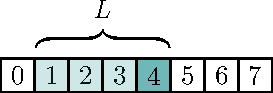
\includegraphics{imagenes/subarray_product_across.pdf}
	\caption{Ejemplo de subarreglo atravesando ambas mitades con $L = 4$ y $N = 8$.}
	\label{ej4:fig:subarray}
\end{figure}

En la Figura \ref{ej4:fig:subarray} se tienen en color claro los elementos del
subarreglo pertenecientes a la mitad izquierda y en color oscuro los de la
derecha. El algoritmo calcula este producto como \texttt{producto[1]} $\times$
\texttt{producto[4]}, donde \texttt{producto[1]} fue calculado por la mitad
izquierda y \texttt{producto[4]} por la derecha:

\begin{align*}
	\texttt{producto[1]} &= M_1 \times \texttt{producto[2]} =
	M_1 \times \left(M_2 \times \texttt{producto[3]}\right) =
	M_1 \times \left(M_2 \times M_3\right) \\
	\texttt{producto[4]} &= M_4
\end{align*}

Es así como la operación responsable de analizar si existe el subarreglo
atravesando ambas mitades pasa a tener un costo $\ord(N)$ ya que únicamente
realiza $\ord(L)$ productos de factores que ya posee generados.

A continuación se presenta el pseudocódigo del algoritmo que resuelve el problema:

\begin{algorithm}[H]
	\caption{Producto subarreglo de matrices}
	\Input{Enteros positivos $N$ y $L$, índices $i$ y $j$, bandera
		\emph{esMitadDerecha} indicando en qué mitad está corriendo la función,
		una matriz $M$ y un arreglo de matrices de longitud $N$ pertenecientes a
		$\mathbb{Z}_{10007}^{3 \times 3}$.}
	\Output{Devuelve \texttt{true} en caso de existir un subarreglo de longitud
		$L$ cuyo producto sea igual a $M$, \texttt{false} caso contrario.}
	\eIf{$N == 1$} {
		\If{$L == 1$ y el único elemento del arreglo es igual a $M$} {
			\Return{\texttt{true}} \;
		}
	}
	{
		\eIf{$L \leq N$} {
			$mitad$ $\gets$ $\frac{N}{2}$ \;
			$derechaResuelve$ $\gets$ llamada recursiva con $N = N - mitad$, $i =
			i + mitad$ \;
			$izquierdaResuelve$ $\gets$ llamada recursiva con $N = mitad$, $j = i
			+ mitad$ \;
			\eIf{$derechaResuelve$ ó $izquierdaResuelve$} {
				\Return{\texttt{true}} \;
			}
			{
				\eIf{el producto existe atravesando ambas mitades} {
					\Return{\texttt{true}} \;
				}
				{
					\eIf{\emph{esMitadDerecha}} {
						calcular y guardar el producto de matrices de $i$ a $j$ \;
					}
					{
						calcular y guardar el producto de matrices de $j$ a $i$ \;
					}
				}
			}
		}
		{
			\eIf{\emph{esMitadDerecha}} {
				calcular y guardar el producto de matrices de $i$ a $j$ \;
			}
			{
				calcular y guardar el producto de matrices de $j$ a $i$ \;
			}
		}
	}

	\Return{\texttt{false}} \;
\end{algorithm}

\subsection{Demostración de correctitud}

Para demostrar que el algoritmo desarrollado es correcto se debe probar que el
mismo responde \texttt{true} si y sólo si existe el subarreglo buscado.

La misma se realizará mediante inducción sobre el valor de $N$ dado un $L$ fijo.

\subsubsection*{Caso base}

Cuando $N = 1$ si $L = 1$ y el único elemento disponible del arreglo corresponde
al producto buscado entonces se cumple lo pedido ya que la solución es la matriz
en esta posición. Caso contrario devuelve \texttt{false} ya que con que no se
cumpla cualquiera de las condiciones anteriores la matriz en tal posición no es
el subarreglo buscado.

\subsubsection*{Paso inductivo}

Suponemos que el algoritmo funciona para arreglos de hasta tamaño $N$ inclusive,
queremos ver que lo hace para $N + 1$.

Primero que nada, si $L > N + 1$ automáticamente sabemos que no existe tal
arreglo, por lo tanto hasta acá el código desarrollado se comporta de la forma
esperada.

Si $L \leq N + 1$ entonces el mismo se llamará de forma recursiva en las mitades
de tamaño $\frac{N + 1}{2}$ y $N - \frac{N + 1}{2}$ respectivamente. Por
hipótesis inductiva, como sabemos que el algoritmo funciona para arreglos de
longitud menor o igual a $N$ en particular lo hace para $\frac{N + 1}{2}$ y $N -
\frac{N + 1}{2}$. De esta manera el mismo nos puede decir si el subarreglo de
longitud $L$ existe en alguna de las dos mitades, si lo hace en cualquiera de
las dos, devuelve \texttt{true}. Caso contrario, es necesario ver si existe
atravesando ambas mitades. Para ello se realiza el producto de todo subarreglo
de longitud $L$ que esté repartido entre ambas mitades. Si uno de estos
subarreglos cumple lo pedido entonces el programa da \texttt{true}, si no
entonces el mismo no existe para $N + 1$. Esto se debe a que si no existe
atravesando las dos mitades debía existir en alguna de las dos, pero estábamos
asumiendo el caso donde las llamadas recursivas dieron \texttt{false}, con lo
cual efectivamente no quedan más lugares donde buscar el producto.

De esta forma queda demostrado que para un $L$ y cualquier $N$ el algoritmo
encuentra el subarreglo buscado en caso de existir. Dado que no realizamos
ninguna suposición sobre $L$ podemos extender sin pérdida de generalidad la
demostración a cualquier valor del mismo.

\subsection{Complejidad teórica}

Dado que se trata de un problema resuelto mediante \emph{Divide \& Conquer} es
posible utilizar el Teorema Maestro para calcular su complejidad teórica. El
mismo define la siguiente recurrencia para caracterizar estos problemas:

\begin{equation*}
	T\left(n\right) = a \times T\left(\frac{n}{b}\right) + f\left(n\right)
\end{equation*}

Para este ejercicio, $n$ corresponde al tamaño del arreglo $N$, $a = 2$ y $b = 2$ ya que se divide el problema en dos y se
deben recorrer ambas mitades, y $f\left(n\right)$ corresponde a la unión que en
nuestro caso es el cálculo de productos de matrices que en la Sección
\ref{ej4:sol} vimos que tenía un costo lineal sobre el tamaño de $N$.

Una de las cotas que ofrece el Teorema Maestro es la siguiente:

\begin{equation*}
	f\left(n\right) \in \Theta\left(n^{\log_b\left(a\right)}\right)
	\implies T\left(n\right) \in \Theta\left(n^{\log_b\left(a\right)} \times
	\log\left(n\right)\right)
\end{equation*}

Como tenemos $a = b = 2$, $\log_b\left(a\right) = 1$ y se cumple
$f\left(n\right) \in \Theta\left(n\right)$. Por lo tanto, la complejidad del
algoritmo está dada por:

\begin{equation*}
	T\left(n\right) \in \Theta\left(n \times \log\left(n\right)\right)
\end{equation*}

Queda demostrado entonces que la complejidad teórica del algoritmo cumple con lo
requerido por el ejercicio resultando en $\Theta\left(n \times
\log\left(n\right)\right)$.

